% Appendix B: Failure cases
\section{Failure cases}
\label{app:failures}

Table~\ref{tab:failure_cases} lists the two stress-test runs where
\ISR underperforms global census.
Both occur at $\sigma = 3.0$, the broadest initial-condition spread.

\begin{table}[t]
  \centering
  \caption{Failure cases: ISR underperforms global census. Both cases occur at $\sigma=3.0$, the broadest initial-condition spread.}
  \label{tab:failure_cases}
  \begin{tabular}{lccccc}
    \toprule
    $\sigma$ & Seed & ISR KL & Global KL & Ratio & Possible cause \\
    \midrule
    3.0 & 13 & 0.0007 & 0.0005 & 0.68 & Broad initial spread samples vacua far from $x_0$; kernel overlap is thin. \\
    3.0 & 14 & 0.0012 & 0.0010 & 0.89 & Broad initial spread samples vacua far from $x_0$; kernel overlap is thin. \\
    \bottomrule
  \end{tabular}
\end{table}


In these runs, the broad initial spread causes many trajectories to sample
vacua far from $x_0$, reducing the effective sample of local sectors.
The Gaussian kernel assigns low weight to distant sectors, and the resulting
measure fluctuates more than the global census, which includes all sectors
regardless of distance.

Fig.~\ref{fig:failure_cases} shows the full $\sigma = 3.0$ distribution
of KL values by seed.

\begin{figure}[t]
  \centering
  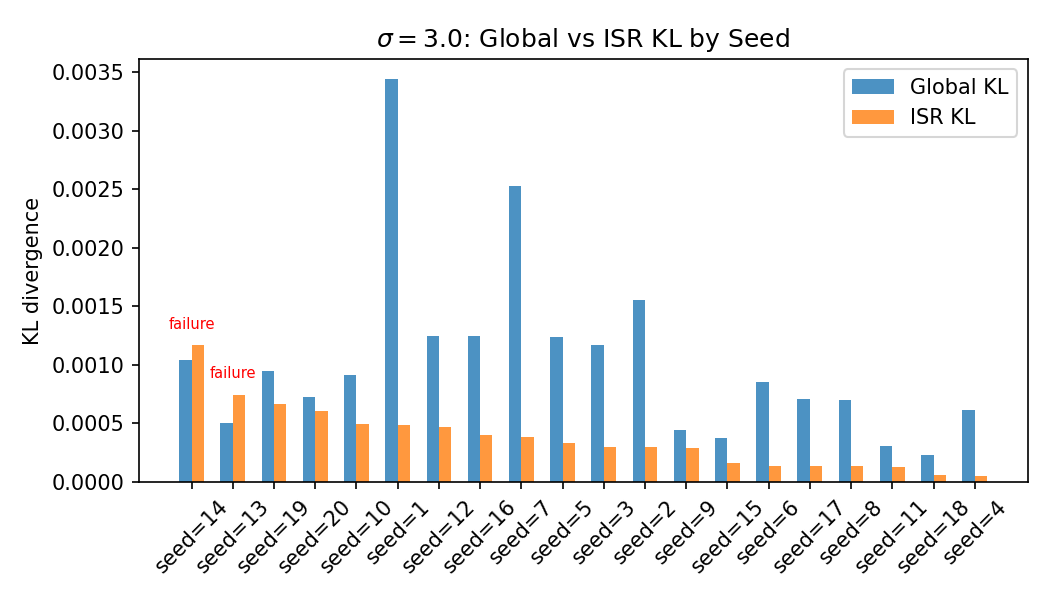
\includegraphics[width=\columnwidth]{figures/fig_08_failure_cases_sigma3.png}
  \caption{KL divergence at $\sigma = 3.0$ for global census and \ISR
  by seed. Two seeds (13 and 14) show \ISR above global.}
  \label{fig:failure_cases}
\end{figure}

\subsection{Diagnostics for both failure cases}

Table~\ref{tab:failure_diagnostics} shows diagnostic metrics for both failure
seeds alongside the non-failure mean at $\sigma=3.0$.
The diagnostics are similar across all three columns: both failure seeds have
$N_{\rm eff}/N$ near 0.48--0.49 and weighted mass in the $x_0$ basin in the
55--59\% range, comparable to the non-failure mean.
The failures are not driven by dramatically different diagnostics but by
borderline cases where the ISR KL divergence slightly exceeds the global
census value by a small margin.

\begin{table*}[t]
  \centering
  \caption{Diagnostic metrics for failure seeds 13 and 14
  ($\sigma=3.0$, $\ell=1.0$, Gaussian kernel) compared with non-failure mean
  at $\sigma=3.0$.}
  \label{tab:failure_diagnostics}
  \small
  \begin{tabular}{lccc}
    \toprule
    Metric & Seed 13 & Seed 14 & Non-failure mean \\
    \midrule
    Effective sample size $N_{\rm eff}$ & 977 & 960 & 963 \\
    $N_{\rm eff} / N$ & 0.49 & 0.48 & 0.48 \\
    Weighted mass in $x_0$ basin & 58.8\% & 54.7\% & 57.7\% \\
    Vacuum distribution entropy & 0.94 nats & 0.97 nats & 0.95 nats \\
    Top vacuum probability & 58.8\% & 54.7\% & 57.7\% \\
    Basin exception rate ($d < \ell$) & 0.0\% & 0.0\% & 0.0\% \\
    Weight concentration $\max(w) / \sum w$ & $1.58\times10^{-3}$ & $1.63\times10^{-3}$ & $1.58\times10^{-3}$ \\
    \bottomrule
  \end{tabular}
\end{table*}

These failures are informative: they show that locality weighting is not
universally beneficial and that broad initial-condition spreads can dilute
the signal. Reporting them honestly strengthens rather than weakens the
analysis.
